\section{擬似乱数}

\begin{frame}[t,fragile]{乱数}
  \begin{itemize}
    \setlength{\itemsep}{1em}
  \item 自然乱数 (ハードウェア乱数)
    \begin{itemize}
    \item さいころ, コイン, ルーレット, 核分裂反応, 熱雑音, ショット雑音 ...
    \end{itemize}
  \item モンテカルロシミュレーションにおける必要条件
    \begin{itemize}
    \item 多数の乱数が必要
    \item ポータビリティ
    \item 生成速度
    \item 再現性
    \end{itemize}
  \item 擬似乱数 (pseudo random number)
    \begin{itemize}
    \item 計算機でプログラムに従って生成
    \item 分布の一様性, 相関, 周期に注意する必要あり
    \end{itemize}
  \end{itemize}
\end{frame}

\begin{frame}[t,fragile]{擬似乱数発生器}
  \begin{itemize}
    %\setlength{\itemsep}{1em}
  \item 最も簡単な乱数発生器:線形合同法 (linear congruential method)
    \[
    x_{n+1} = (ax_n+c) \ \mbox{mod} \ m
    \]
  \item 例) $a = 65539$, $c = 0$, $m = 2147483648$ (周期 $m-1$)
  \item 少しだけ異なる初期値 $(x0 = 1, 2, 3)$ から始めた場合
  \resizebox{!}{.35\textheight}{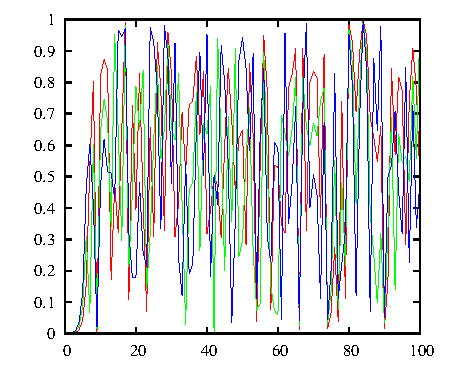
\includegraphics{image/lcg-1.pdf}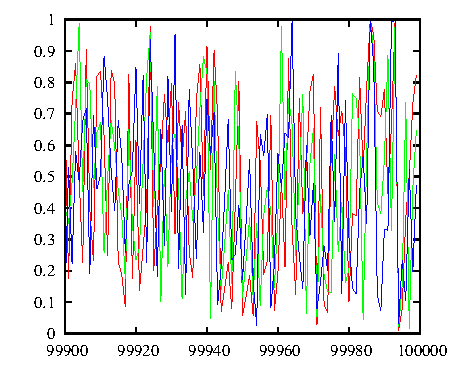
\includegraphics{image/lcg-2.pdf}}
  \item 数十ステップ進むとバラバラな振舞い ⇒ カオス的
  \end{itemize}
\end{frame}

\begin{frame}[t,fragile]{擬似乱数生成器における相関}
  \begin{itemize}
    %\setlength{\itemsep}{1em}
  \item 合同乗算法で多次元超立方体中に「ランダムに」点を打つと、それらの点は全て比較的小数の等間隔に並んだ超平面の上にのってしまう (多次元疎結晶構造)
  \resizebox{!}{.35\textheight}{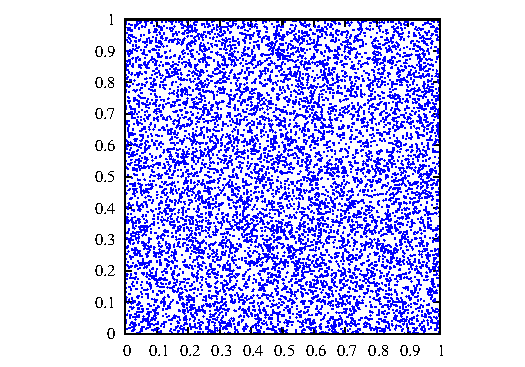
\includegraphics{image/lcg-2d.pdf}}
  \resizebox{!}{.35\textheight}{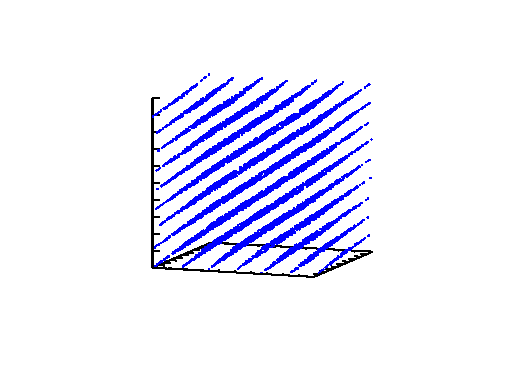
\includegraphics{image/lcg-3d.pdf}}
  \item 計算式に従って生成するため、必ず何らかの相関は残る
  \item できる限り相関が少なく周期の長い、理想的な乱数の開発が続けられている
    \begin{itemize}
    \item 現時点で、標準的な乱数発生器:メルセンヌ・ツイスター
    \item 周期 $2^{19937}-1$、高速、日本製! (例: \href{https://github.com/todo-group/computer-experiments/blob/master/exercise/monte_carlo/random.c}{example-2-L2/random.c})
    \end{itemize}
  \end{itemize}
\end{frame}

\begin{frame}[t,fragile]{乱数発生器の選び方}
  \begin{itemize}
    %\setlength{\itemsep}{1em}
  \item 万能乱数発生器は存在しない
  \item 生成された乱数のもつ性質について, 様々な数学的に厳密な証明, 多くのテスト結果がすでに存在するが, 特定のシミュレーションに使った場合の結果については何も保証してくれない
  \item 自分で乱数発生器を「発明」してはいけない
  \item 自分で乱数発生器をプログラムしてはいけない (既存のライブラリを使う)
  \item 初期化(種の設定)を正しく行う
  \item 実際にそれらしい乱数が生成されているか, 目でみて確認する
  \item 二種類以上の乱数発生器を使ってみて, 互いに一致する結果が出るかどうか確認する
  \end{itemize}
\end{frame}

\begin{frame}[t,fragile]{様々な分布}
  \begin{itemize}
    %\setlength{\itemsep}{1em}
  \item 乱数発生器は通常、一様な整数乱数あるいは実数乱数を生成
  \item 一様分布以外の分布にしたがう乱数の発生方法の代表例
  \item 逆関数法
    \begin{itemize}
      \item 確率分布関数$F(x)$の逆関数$F^{-1}(y)$ と(0,1)の一様乱数$u$から $v=F^{-1}(u)$
      \item 例: 指数分布 $p(x) = \frac{1}{\mu} e^{-x/\mu}$

      $F(x) = 1 - e^{-x/\mu}$ \ \ \ $F^{-1}(y) = - \mu \log(1-y)$
      \item 一般の確率分布関数について逆関数を求めるのは困難
    \end{itemize}
  \item 棄却法
    \begin{itemize}
      \item 確率密度関数を完全に囲むような箱を用意し、その箱の中で一様乱数を生成
      \item 確率密度関数の下側の点が生成されたら、その$x$座標を乱数として採用。上側の点の場合には再度生成
      \item もとの確率密度関数よりも箱が大きくなりすぎると非効率
    \end{itemize}
  \end{itemize}
\end{frame}
